\documentclass[aspectratio=169,handout]{beamer}
\usepackage{borelian}

\begin{document}
  \classtitle{16}{Reducción de dimensionalidad}{15 de enero de 2026}

  \begin{frame}[fragile]{Motivación}
    En muchos problemas de Machine Learning, los datos pueden tener una gran cantidad de dimensiones (columnas en un \mintinline{python}{pd.DataFrame}). Esto afecta principalmente en dos áreas:
    \pause
    \begin{itemize}
      \item \underline{Maldición de la dimensionalidad}: las distancias empiezan a ser parecidas en espacios de muchas dimensiones. Esto afecta a algoritmos basados en distancias, como $k$-NN y $K$-\emph{Means}.
      \pause
      \item \underline{Visualización de información}: el ser humano, biológicamente, está limitado a ver en dos dimensiones y ``construir'' una sensación de profundidad, lo que añade una tercera dimensión. ¿Cómo interpretaríamos datos que pueden ser graficados únicamente en más de $3$ dimensiones?
    \end{itemize} 

    \pause
    \begin{figure}[H]
  \centering
  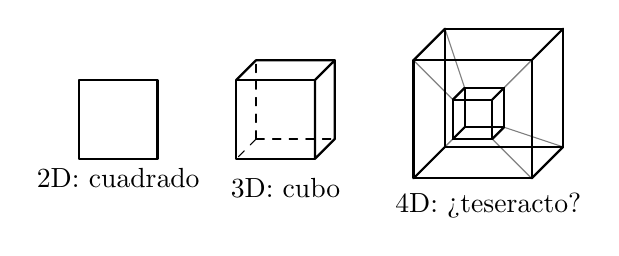
\begin{tikzpicture}[scale=0.5,line join=round,line cap=round,x=1cm,y=1cm]
    \begin{scope}[shift={(0,0)}]
      \draw[thick] (0,0) rectangle (2,2);
      \node at (1,-0.5) {2D: cuadrado};
    \end{scope}

    \begin{scope}[shift={(4,0)}]
      % Hidden edges
      \draw[dashed] (0.5,0.5) -- (2.5,0.5);
      \draw[dashed] (0.5,0.5) -- (0.5,2.5);
      \draw[dashed] (0.5,0.5) -- (0,0);
      
      % Visible faces
      \draw[thick] (0,0) rectangle (2,2);
      \draw[thick] (2,0) -- (2.5,0.5) -- (2.5,2.5) -- (2,2) -- cycle;
      \draw[thick] (0,2) -- (0.5,2.5) -- (2.5,2.5);
      
      \node at (1.25,-0.75) {3D: cubo};
    \end{scope}

    \begin{scope}[shift={(9,0)}]
      % Inner cube (smaller)
      \coordinate (A1) at (0.5,0.5); \coordinate (B1) at (1.5,0.5);
      \coordinate (C1) at (1.5,1.5); \coordinate (D1) at (0.5,1.5);
      \coordinate (A2) at (0.8,0.8); \coordinate (B2) at (1.8,0.8);
      \coordinate (C2) at (1.8,1.8); \coordinate (D2) at (0.8,1.8);

      % Outer cube (larger)
      \coordinate (E1) at (-0.5,-0.5); \coordinate (F1) at (2.5,-0.5);
      \coordinate (G1) at (2.5,2.5);   \coordinate (H1) at (-0.5,2.5);
      \coordinate (E2) at (0.3,0.3);   \coordinate (F2) at (3.3,0.3);
      \coordinate (G2) at (3.3,3.3);   \coordinate (H2) at (0.3,3.3);

      % Connecting inner and outer vertices
      \foreach \from/\to in {A1/E1, B1/F1, C1/G1, D1/H1, A2/E2, B2/F2, C2/G2, D2/H2}
        \draw[gray, thin] (\from) -- (\to);

      % Draw Inner Cube
      \draw[thick] (A1) -- (B1) -- (C1) -- (D1) -- cycle;
      \draw[thick] (A2) -- (B2) -- (C2) -- (D2) -- cycle;
      \foreach \from/\to in {A1/A2, B1/B2, C1/C2, D1/D2} \draw[thick] (\from) -- (\to);

      % Draw Outer Cube
      \draw[thick] (E1) -- (F1) -- (G1) -- (H1) -- cycle;
      \draw[thick] (E2) -- (F2) -- (G2) -- (H2) -- cycle;
      \foreach \from/\to in {E1/E2, F1/F2, G1/G2, H1/H2} \draw[thick] (\from) -- (\to);

      \node at (1.4,-1.2) {4D: ¿teseracto?};
    \end{scope}
  \end{tikzpicture}
\end{figure}
  \end{frame}

  \begin{frame}{Maldición de la dimensionalidad}
    Veremos un ejemplo sencillo para entender este concepto.

    \pause
    \begin{exampleblock}{Características sociales del curso}
      Queremos comparar características entre estudiantes de este curso. Si consideramos sólo una variable, como la \texttt{altura}, es relativamente sencillo encontrar estudiantes parecidos.

      \pause
      Si a la comparación le sumamos la \texttt{edad}, la probabilidad de encontrar estudiantes similares disminuye, pero aún es posible.

      \pause
      Si nos vamos al extremo, considerando $100$ variables distintas, ya es \underline{casi imposible} encontrar a dos estudiantes que sean similares en todas las dimensiones, incluso en varias de ellas.
      
      \pause
      \textbf{Esto ilustra cómo, a medida que aumentamos las dimensiones, los datos tienden a dispersarse y las distancias se vuelven menos significativas.}
    \end{exampleblock}
  \end{frame}

  \begin{frame}{Maldición de la dimensionalidad}
    Para entenderlo, ahora matemáticamente, veamos el siguiente diagrama, donde se indican los puntos centrales $(0.5, 0.5)$ y $(0.5, 0.5, 0.5)$ y el punto más cercano a ellos.
    \vspace{-.4cm}
    \begin{figure}[H]
      \centering
      \includegraphics[width=.9\linewidth]{scripts/09/out/curse_dim.pdf}
    \end{figure}
  \end{frame}

  \begin{frame}{Maldición de la dimensionalidad}
    La razón detrás de que la distancia $d_\text{mín}$ aumente al pasar de un plano 2D a un espacio 3D radica en la fórmula que se ocupa para hacer esta medición.
    \pause
    \begin{itemize}
      \item Para dos dimensiones, es $d = \sqrt{\left(\Delta x\right)^2 + \left(\Delta y\right)^2}$.
      \pause
      \item Para tres dimensiones, es $d = \sqrt{\left(\Delta x\right)^2 + \left(\Delta y\right)^2 + \left(\Delta z\right)^2}$.
    \end{itemize}
    \pause
    En cualquier caso, el agregar la tercera componente $\left(\Delta z\right)^2$ sólo puede aumentar la distancia total $d$, porque $\left(\Delta z\right)^2 \ge 0$. La probabilidad de que este valor sea exactamente cero es muy baja.
  \end{frame}

  \begin{frame}{Algoritmos de reducción de dimensionalidad}
    Enfoquémonos en los algoritmos que nos permiten reducir dimensiones. En esta clase, veremos tres de ellos:
    \pause
    \begin{itemize}
      \item PCA (\emph{Principal Component Analysis}).
      \pause
      \item $t$-SNE ($t$-\emph{distributed Stochastic Neighbor Embedding}).
      \pause
      \item UMAP (\emph{Uniform Manifold Approximation and Projection}).
    \end{itemize}

    \pause
    \begin{block}{Curiosidad}
      No es coincidencia que UMAP tenga ``forzosamente'' la palabra \emph{map} en su nombre. En matemáticas, un mapa es una función que asigna elementos de un conjunto a otro, ¿y qué estamos haciendo acá?
    \end{block}
  \end{frame}

  \begin{frame}{PCA: \emph{Principal Component Analysis}}
    Este algoritmo busca reducir dimensiones manteniendo la mayor cantidad de información explicada posible desde una perspectiva global.
    \pause
    \begin{exampleblock}{Analogía del fotógrafo}
      Imaginen que están fotografiando un paisaje. El mundo real es tridimensional, pero las fotografías reposan sobre un plano bidimensional.

      \pause
      Un buen fotógrafo buscará el mejor ángulo para capturar la esencia del paisaje en su fotografía, que usualmente se obtendrá desde puntos altos, maximizando la cantidad de información visual que puede transmitir en dos dimensiones.

      \pause
      Podemos pensar que cada elemento del paisaje aporta información. Hay algunos que aportan más que otros. Por ejemplo, si sacamos la fotografía mirando a una pared, no capturaremos casi nada de la esencia original.
    \end{exampleblock}
  \end{frame}

  \begin{frame}{PCA: \emph{Principal Component Analysis}}
    La idea que subyace tras este algoritmo es, en esencia, la misma. Hay variables que aportan más información que otras. 
    \pause
    \begin{exampleblock}{Ejemplo geométrico}
      Si tuviésemos variables de largo, anchura y altura, y además el área y el volumen, estas últimas no aportarían información adicional, pues pueden ser calculadas \textbf{directamente} a partir de las otras tres variables.
    \end{exampleblock}
    \pause
    \begin{block}{PCA y correlaciones}
      Naturalmente, variables que estén altamente correlacionadas entre sí aportan información que llamamos redundante. Una forma de identificar las variables que pueden ser eliminadas es analizando la matriz de correlación del problema.
    \end{block}
  \end{frame}

  \begin{frame}[fragile]{Aplicación de PCA}
    Usando la implementación de PCA de Scikit-Learn, podemos ver un ejemplo sencillo de cómo funciona este algoritmo.
    \begin{columns}
      \column{0.475\linewidth}
      \begin{minted}[fontsize=\small]{python}
        >>> import pandas as pd
        >>> from sklearn.decomposition import PCA

        >>> data = pd.DataFrame({
        ...    'Math': [850, 871, 944, ...],
        ...    'Physics': [824, 880, 915, ...] 
        ... })

        >>> pca = PCA(n_components=1)
        >>> pca_result = pca.fit_transform(data)

        >>> pca.explained_variance_ratio_
      \end{minted}

      \hfill
      \column{0.475\linewidth}
      \pause
      \vspace{-.5cm}
      \begin{figure}[H]
        \centering
        \includegraphics[width=\linewidth]{scripts/09/out/pca.pdf}
      \end{figure}
    \end{columns}
  \end{frame}

  \begin{frame}{$t$-SNE: $t$-\emph{distributed Stochastic Neighbor Embedding}}
    Recordemos la analogía de la fotografía para PCA. Esta analogía sugiere que PCA reduce las dimensiones con un enfoque global, porque un buen ángulo de fotografía trataría de capturar la mayor parte del paisaje (p. ej., mirando desde arriba, sin detalles locales).

    \pause
    En contraste, $t$-SNE funciona preservando las relaciones locales de los puntos en altas dimensiones. Es decir, si dos puntos están cerca en el espacio original, deberían permanecer cerca en el espacio reducido.

    \pause
    \begin{block}{¿Por qué se parece tanto a una clusterización?}
      Es cierto que podemos vincular este algoritmo con la idea de clusterización, donde queremos que puntos similares (cercanos) permanezcan juntos. La diferencia radica en que $t$-SNE \textbf{no} asigna etiquetas (es decir, no dice tú eres del grupo $1$, aquel del grupo $2$, etc.), simplemente reduce las dimensiones.
    \end{block}
  \end{frame}

  \begin{frame}{Aplicación de $t$-SNE: MNIST}
    Veamos un ejemplo sencillo usando el conjunto de datos MNIST, que contiene imágenes de dígitos escritos a mano ($0$-$9$). 

    \pause
    A la izquierda, se muestran algunas imágenes del conjunto de datos original, y a la derecha, el resultado de aplicar $t$-SNE (\mintinline{python}{from sklearn.manifold import TSNE}) para reducir las dimensiones a $2$.
    \begin{columns}
      \column{0.475\linewidth}
      \begin{figure}[H]
        \centering
        \includegraphics[width=\linewidth]{days/09/images/mnist.png}
      \end{figure}

      \hfill
      \column{0.475\linewidth}
      \vspace{-.85cm}
      \begin{figure}[H]
        \centering
        \includegraphics[width=.85\linewidth]{scripts/09/out/t-sne.pdf}
      \end{figure}
    \end{columns}
  \end{frame}

  \begin{frame}{UMAP: \emph{Uniform Manifold Approximation and Projection}}
    UMAP (\mintinline{python}{import umap}) es como el ``híbrido'' entre PCA y $t$-SNE. Busca preservar tanto las relaciones locales como las globales en los datos al reducir dimensiones.
    \pause
    \begin{exampleblock}{Volviendo a la vista del paisaje...}
      Si lo pensamos como elementos que podemos identificar en el día a día:
      \pause
      \begin{itemize}
        \item PCA sería la vista satelital: puede visualizar todo, pero sin enfocarse en detalles específicos.
        \pause
        \item $t$-SNE sería el modo ``Street View'', que baja directamente a la calle y muestra detalles locales, sin preocuparse por la vista global.
        \pause
        \item UMAP sería como una vista panorámica desde un dron, que es capaz de capturar, dada la altura que tiene, tanto la vista global como detalles locales.
      \end{itemize}
    \end{exampleblock}    
  \end{frame}

  \begin{frame}{Detalles importantes de estos algoritmos}
    \begin{itemize}
      \item UMAP tiene hiperparámetros que permiten ajustar el equilibrio entre la preservación local y global. Esto permite incluso imitar el resultado que daría $t$-SNE o PCA dependiendo de los valores escogidos.
      \pause
      \item PCA y UMAP son algoritmos que aprenden reglas: tal cual lo vimos en regresión lineal, se aprenden parámetros (que en ese caso eran coeficientes) que permiten transformar nuevos datos.
      \pause
      \item $t$-SNE resuelve un acertijo único por ejecución: no permite transformar nuevos datos directamente, dado que corresponderían a ``otro acertijo''.
    \end{itemize}
  \end{frame}
\end{document}